\documentclass{beamer}
\usepackage{amsmath}
\usepackage[english]{babel} %set language; note: after changing this, you need to delete all auxiliary files to recompile
\usepackage[utf8]{inputenc} %define file encoding; latin1 is the other often used option
\usepackage{csquotes} % provides context sensitive quotation facilities
\usepackage{graphicx} %allows for inserting figures
\usepackage{booktabs} % for table formatting without vertical lines
\usepackage{textcomp} % allow for example using the Euro sign with \texteuro
\usepackage{stackengine}
\usepackage{wasysym}
\usepackage{tikzsymbols}
\usepackage{textcomp}
\newcommand{\bubblethis}[2]{
        \tikz[remember picture,baseline]{\node[anchor=base,inner sep=0,outer sep=0]%
        (#1) {\underline{#1}};\node[overlay,cloud callout,callout relative pointer={(0.2cm,-0.7cm)},%
        aspect=2.5,fill=yellow!90] at ($(#1.north)+(-0.5cm,1.6cm)$) {#2};}%
    }%
\tikzset{face/.style={shape=circle,minimum size=4ex,shading=radial,outer sep=0pt,
        inner color=white!50!yellow,outer color= yellow!70!orange}}
%% Some commands to make the code easier
\newcommand{\emoticon}[1][]{%
  \node[face,#1] (emoticon) {};
  %% The eyes are fixed.
  \draw[fill=white] (-1ex,0ex) ..controls (-0.5ex,0.2ex)and(0.5ex,0.2ex)..
        (1ex,0.0ex) ..controls ( 1.5ex,1.5ex)and( 0.2ex,1.7ex)..
        (0ex,0.4ex) ..controls (-0.2ex,1.7ex)and(-1.5ex,1.5ex)..
        (-1ex,0ex)--cycle;}
\newcommand{\pupils}{
  %% standard pupils
  \fill[shift={(0.5ex,0.5ex)},rotate=80] 
       (0,0) ellipse (0.3ex and 0.15ex);
  \fill[shift={(-0.5ex,0.5ex)},rotate=100] 
       (0,0) ellipse (0.3ex and 0.15ex);}

\newcommand{\emoticonname}[1]{
  \node[below=1ex of emoticon,font=\footnotesize,
        minimum width=4cm]{#1};}
\usepackage{scalerel}
\usetikzlibrary{positioning}
\usepackage{xcolor,amssymb}
\newcommand\dangersignb[1][2ex]{%
  \scaleto{\stackengine{0.3pt}{\scalebox{1.1}[.9]{%
  \color{red}$\blacktriangle$}}{\tiny\bfseries !}{O}{c}{F}{F}{L}}{#1}%
}
\newcommand\dangersignw[1][2ex]{%
  \scaleto{\stackengine{0.3pt}{\scalebox{1.1}[.9]{%
  \color{red}$\blacktriangle$}}{\color{white}\tiny\bfseries !}{O}{c}{F}{F}{L}}{#1}%
}
\usepackage{fontawesome} % Social Icons
\usepackage{epstopdf} % allow embedding eps-figures
\usepackage{tikz} % allows drawing figures
\usepackage{amsmath,amssymb,amsthm} %advanced math facilities
\usepackage{lmodern} %uses font that support italic and bold at the same time
\usepackage{hyperref}
\usepackage{tikz}
\hypersetup{
    colorlinks=true,
    linkcolor=blue,
    filecolor=magenta,      
    urlcolor=blue,
}
\usepackage{tcolorbox}
%add citation management using BibLaTeX
\usepackage[citestyle=authoryear-comp, %define style for citations
    bibstyle=authoryear-comp, %define style for bibliography
    maxbibnames=10, %maximum number of authors displayed in bibliography
    minbibnames=1, %minimum number of authors displayed in bibliography
    maxcitenames=3, %maximum number of authors displayed in citations before using et al.
    minnames=1, %maximum number of authors displayed in citations before using et al.
    datezeros=false, % do not print dates with leading zeros
    date=long, %use long formats for dates
    isbn=false,% show no ISBNs in bibliography (applies only if not a mandatory field)
    url=false,% show no urls in bibliography (applies only if not a mandatory field)
    doi=false, % show no dois in bibliography (applies only if not a mandatory field)
    eprint=false, %show no eprint-field in bibliography (applies only if not a mandatory field)
    backend=biber %use biber as the backend; backend=bibtex is less powerful, but easier to install
    ]{biblatex}
\addbibresource{../mybibfile.bib} %define bib-file located one folder higher


\usefonttheme[onlymath]{serif} %set math font to serif ones

\definecolor{beamerblue}{rgb}{0.2,0.2,0.7} %define beamerblue color for later use

%%% defines highlight command to set text blue
\newcommand{\highlight}[1]{{\color{blue}{#1}}}


%%%%%%% commands defining backup slides so that frame numbering is correct

\newcommand{\backupbegin}{
   \newcounter{framenumberappendix}
   \setcounter{framenumberappendix}{\value{framenumber}}
}
\newcommand{\backupend}{
   \addtocounter{framenumberappendix}{-\value{framenumber}}
   \addtocounter{framenumber}{\value{framenumberappendix}}
}

%%%% end of defining backup slides

%Specify figure caption, see also http://tex.stackexchange.com/questions/155738/caption-package-not-working-with-beamer
\setbeamertemplate{caption}{\insertcaption} %redefines caption to remove label "Figure".
%\setbeamerfont{caption}{size=\scriptsize,shape=\itshape,series=\bfseries} %sets figure  caption bold and italic and makes it smaller


\usetheme{Boadilla}

%set options of hyperref package
\hypersetup{
    bookmarksnumbered=true, %put section numbers in bookmarks
    naturalnames=true, %use LATEX-computed names for links
    citebordercolor={1 1 1}, %color of border around cites, here: white, i.e. invisible
    linkbordercolor={1 1 1}, %color of border around links, here: white, i.e. invisible
    colorlinks=true, %color links
    anchorcolor=black, %set color of anchors
    linkcolor=beamerblue, %set link color to beamer blue
    citecolor=blue, %set cite color to beamer blue
    pdfpagemode=UseThumbs, %set default mode of PDF display
    breaklinks=true, %break long links
    pdfstartpage=1 %start at first page
    }


% --------------------
% Overall information
% --------------------
\title[Principios de Economía]{Principios de Economía}
\date{}
\author[Ertola y Sturzenegger]{Gabriela Ertola y Federico Sturzenegger }
\vspace{0.4cm}
\institute[]{Universidad de San Andrés \\
2022} 


\begin{document}

\begin{frame}
\frametitle{Principios de Economía
\centering
\\ \vspace{12mm} Política Económica}
\centering
 \\ \vspace{12mm} %5 de agosto, 2021 \vspace{5mm} \\ 
\includegraphics[scale=0.25]{Figures/logoUDESA.jpg} 

\end{frame}


\begin{frame}{Política Monetaria en el mundo clásico}
 
 \begin{center}
\begin{figure}[H]
\renewcommand{\figurename}{Figure}
\begin{center}
    \begin{minipage}[b]{0.45\textwidth}
        \begin{center}
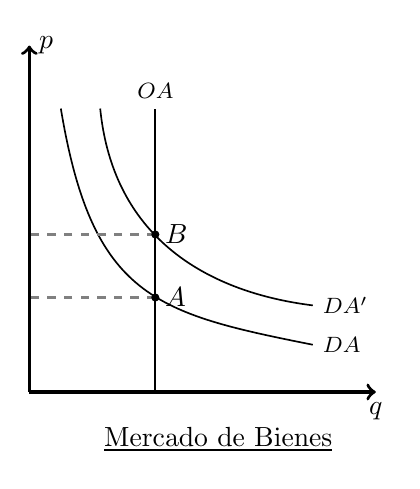
\begin{tikzpicture}[scale=0.4]
\draw[very thick,<-] (0,11)--(0,0);
\draw[very thick,->] (0,0)--(11,0) node[below]{$q$};
\node[right] at (0,11) {$p$};

\node[] at(6,-1.5) {\underline{Mercado de Bienes}};
\draw[semithick] (1,9).. controls (2,3) and (4, 2.5) .. (9, 1.5) node [right]{\footnotesize $DA$};
\draw[semithick] (2.25,9).. controls (2.75,4) and (7, 3) .. (9, 2.75) node [right]{\footnotesize $DA'$};
\draw[semithick](4, 0)--(4, 9) node [above]{\footnotesize $OA$};
\draw[thick, gray, dashed] (4,3)--(0,3);
\draw[thick, gray, dashed] (4,5)--(0,5);
   \draw[fill] (4,3) circle [radius =0.11] node[right] {$A$}; 
      \draw[fill] (4,5) circle [radius =0.11] node[right] {$B$}; 
\end{tikzpicture}
\end{center}
     \end{minipage}
  %  \hfill
    \begin{minipage}[b]{0.45\textwidth}
    \begin{center}
\begin{tikzpicture}[scale=0.4]
\draw[very thick,<-] (0,11) node[above]{$i$}--(0,0);
\draw[very thick,->] (0,0)--(11,0) node[below]{$M$};
\node[right] at (0,11) {};


\node[] at(6,-1.5) {\underline{Mercado de Dinero}};
\draw[semithick] (1,9).. controls (2,3) and (4, 2.5) .. (9, 1.5) node [right]{\footnotesize $M^{d}$};
\draw[semithick] (2.25,9).. controls (2.75,4) and (7, 3) .. (9, 2.75) node [right]{\footnotesize $M^{d^{'}}$};
\draw[semithick](3.5, 0)--(3.5, 9) node [above]{\footnotesize $M^{o}$};
 \draw[semithick](6.5, 0)--(6.5, 9) node [above]{\footnotesize $M^{o}'$};
 \draw[thick, gray, dashed] (6.5,3.35)--(0,3.35);
   \draw[fill] (3.5,3.35) circle [radius =0.11] node[right] {$A$}; 
      \draw[fill] (6.5,3.35) circle [radius =0.11] node[right] {$B$}; 
\end{tikzpicture}
\end{center}
    \end{minipage}
\end{center}
\vspace{0.7cm}
\label{fig:C35.4}
\end{figure}
\end{center} 

 
\end{frame}



%---------------------------------------------------------------------------%

\begin{frame}{Política monetaria en el mundo clásico}
\begin{itemize}
    \item “Aumenta la demanda agregada” al meter liquidez en el sistema 
    \item Pero el producto está dado por la oferta agregada
    \item Por lo que el aumento en la demanda presiona sobre los precios
    \item Lo que lleva a que los precios aumenten proporcionalmente a lo que aumentó la cantidad de dinero
    \item Oferta y demanda de dinero simplemente se corren para encontrar el equilibrio en el mismo nivel.
    \item $\uparrow M V(i)=\uparrow P Y$ 
    \item Dicotomía clásica (“Neutralidad del dinero”) - $(Y \text { e } i \text { constante, } M \rightarrow P)$
    \end{itemize}
 

\end{frame}

%---------------------------------------------------------------------------%

\begin{frame}{¿Cómo se recauda el impuesto inflacionario?}

    \begin{itemize}
        \item El gobierno emite un dinero
        \item Esto aumenta lo precios
        \item Ese aumento de precios hace que los tenedores de pesos puedan consumir menos.
        \item De esa manera parte del producto lo apropia el Estado
    \end{itemize}
    
\end{frame}

%---------------------------------------------------------------------------%

\begin{frame}{Política monetaria en el mundo keynesiano}
  
\begin{center}
\begin{figure}[H]
\renewcommand{\figurename}{Figure}
\begin{center}
    \begin{minipage}[b]{0.45\textwidth}
        \begin{center}
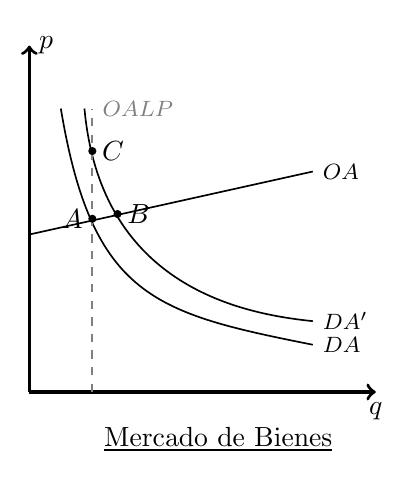
\begin{tikzpicture}[scale=0.4]
\draw[very thick,<-] (0,11)--(0,0);
\draw[very thick,->] (0,0)--(11,0) node[below]{$q$};
\node[right] at (0,11) {$p$};


\node[] at(6,-1.5) {\underline{Mercado de Bienes}};
\draw[semithick] (1,9).. controls (2,3) and (4, 2.5) .. (9, 1.5) node [right]{\footnotesize $DA$};
\draw[semithick] (1.75,9).. controls (2.25,3.5) and (6.5,2.5) .. (9, 2.25) node [right]{\footnotesize $DA'$};
\draw[semithick](0, 5)--(9, 7) node [right]{\footnotesize $OA$};
 \draw[thick, gray, dashed] (2,0)--(2,9) node [right]{\footnotesize $OALP$};
   \draw[fill] (2,5.5) circle [radius =0.11] node[left] {$A$}; 
  \draw[fill] (2.8,5.65) circle [radius =0.11] node[right] {$B$}; 
  \draw[fill] (2,7.65) circle [radius =0.11] node[right] {$C$}; 
 
\end{tikzpicture}
\end{center}
     \end{minipage}
  %  \hfill
    \begin{minipage}[b]{0.45\textwidth}
    \begin{center}
\begin{tikzpicture}[scale=0.4]
\draw[very thick,<-] (0,11) node[above]{$i$}--(0,0);
\draw[very thick,->] (0,0)--(11,0) node[below]{$M$};
\node[right] at (0,11) {};

\node[] at(6,-1.5) {\underline{Mercado de Dinero}};
\draw[semithick] (1,9).. controls (2,3) and (4, 2.5) .. (9, 1.5) node [right]{\footnotesize $M^{d}$};
\draw[semithick] (1.75,9).. controls (2.25,3) and (6.75, 2.5) .. (9, 2.15) node [right]{\footnotesize $M^{d^{'}}$};
\draw[semithick, gray, dashed] (2.5,9).. controls (2.25,3.7) and (6.75, 3.5) .. (9, 2.9) node [right]{\footnotesize $M^{d^{''}}$};
\draw[semithick](3.5, 0)--(3.5, 9) node [above]{\footnotesize $M^{o}$};
 \draw[semithick](6.5, 0)--(6.5, 9) node [above]{\footnotesize $M^{o}'$};
 \draw[semithick](6.5, 0)--(6.5, 9) node [above]{\footnotesize $M^{o}'$};


 \draw[thick, gray, dashed] (3.5,3.35)--(0,3.35);
 \draw[thick, gray, dashed] (6.5,2.625)--(0,2.625);

  \draw[fill] (3.35,3.35) circle [radius =0.11] node[right] {$A$}; 
  \draw[fill] (6.5,2.625) circle [radius =0.11] node[right] {$B$}; 
   \draw[fill] (6.5,3.35) circle [radius =0.11] node[right] {$C$}; 
\end{tikzpicture}
\end{center}
    \end{minipage}
\end{center}
\vspace{0.7cm}
\label{fig:C35.5}
\end{figure}
\end{center}   
\end{frame}


%---------------------------------------------------------------------------%
\begin{frame}{Política monetaria en el mundo keynesiano}

\begin{itemize}
    \item Ahora “aumenta la demanda agregada” pero ahora esto baja la tasa de interés y lleva a un aumento en el producto.
    \item El dinero excedente reduce la tasa de interés en el mercado de crédito
    \item $\uparrow M V(i) \downarrow=\bar{P} Y \uparrow$
    \item (P constante $, M \rightarrow i, i \rightarrow Y)$
\end{itemize}
 

\end{frame}

%---------------------------------------------------------------------------%

\begin{frame}{¿Es efectiva la política monetaria?}

    \begin{itemize}
        \item Depende del contexto si los precios se mueven rápido no va a lograr mucho, si los precios son "rígidos" tendrá más impacto. 
        \item En definitiva es una cuestión de contexto.
        \item Podríamos presumir que la política monetaria en Argentina sería menos efectiva que en los EEUU

    \end{itemize}
    
\end{frame}

%---------------------------------------------------------------------------%

\begin{frame}{¿Cómo funciona la política monetaria?}
    
    \centering\includegraphics[width=11cm]{P81.png}\

\end{frame}

\begin{frame}{}
\centering 	\huge \textbf{Política fiscal} 
\vspace{2mm}
\hrule
\end{frame}


\begin{frame}{¿Cómo funciona la política fiscal?}
    \begin{itemize}
        \item El análisis de la política fiscal es mucho más complejo por una serie de motivos:
        \begin{itemize}
            \item La política fiscal expansiva genera aumentos de la demanda agregada 
            \item Pero la política fiscal requiere financiamiento
            \begin{itemize}
                \item Necesitamos entender cómo puede financiar el Gobierno para hacer uso de este instrumento
            \end{itemize}
            \item Hay efectos expulsión (“crowding out”) vía la tasa de interés (que no aparecían con la política monetaria)
        \end{itemize}
        \vspace{2mm}
        \item La combinación de estos tres factores nos dará el efecto neto de la política fiscal sobre la demanda agregada
    \end{itemize}
\end{frame}

\begin{frame}{¿Cómo puede financiar el gasto un gobierno?}
    \begin{itemize}
        \item Existen cuatro mecanismos básicos para financiar la política fiscal:
        \begin{itemize}
            \item Hacer emisión monetaria 
            \item Aumentar los impuestos
            \item Pedir deuda interna
            \item Pedir deuda externa 
        \end{itemize}
        \vspace{2mm}
        \item Cada uno de estos implicará distintos mecanismos sobre la demanda agregada
    \end{itemize}
\end{frame}


\begin{frame}{El efecto “financiamiento” sobre el consumo: impuestos}
    
    \begin{itemize}
        \item Si aumenta el gasto público financiado enteramente con impuestos: ¿cuánto cae el consumo privado?
        \begin{itemize}
            \item Cae el consumo que esos impuestos desplazan
            \item Si los impuestos son permanentes la caída del consumo debiera ser el 100\% del aumento de los impuestos (primer caso)
            \item La caída del consumo es menor si se piensa que es transitorio y podría aumentar el producto en le corto plazo (segundo y tercer caso)
            \item Lo cierto es que el efecto de la política fiscal se modera sustancialmente cuando se tiene en cuenta el financiamiento
        \end{itemize}
        \end{itemize}

\end{frame}

\begin{frame}{El efecto “financiamiento” sobre el consumo: deuda }
    
    \begin{itemize}
        \item Si aumenta el gasto público financiado con deuda: ¿cuánto cae el consumo privado?
        \begin{itemize}
            \item En principio podríamos pensar que nada 
            \item Pero si existe “equivalencia ricardiana”, cae igual que si se financia con impuestos (casos anteriores)
            \item Y hay crowding out también si hay un aumento en la tasa de interés 
        \end{itemize}
    \end{itemize}

\end{frame}
%---------------------------------------------------------------------------%

\begin{frame}{Ejemplo de equivalencia ricardiana}
    
\begin{itemize}
    \item Supongamos dos periodos en los que el individuo tiene ingresos de 1000 y 1000
    \item El gobierno quiere gastar 100 y 100 
    \item Lo financia con deuda en el primer periodo y la tasa de interés es 10\%
    \item El agente enfrenta impuestos de 0 y 210
    \item Si consume su ingreso consumiría 1000 y 790 
    \item ¿Qué pasa si ahorra 100 en el primero período?
    \item Ahora puede consumir 900 y 900 (que es mejor que 1000 y 790)
    \item Pero 900 y 900 ¡es lo mismo que si el gobierno hubiera financiado los 100 con impuestos! 
\end{itemize}

\end{frame}

%---------------------------------------------------------------------------%

\begin{frame}{El efecto expulsión (“crowding out”)}

    \begin{itemize}
    \footnotesize\item Tiene dos componentes:
        \begin{itemize}
        \scriptsize\item El menor ingreso neto implica menor ahorro lo cual reduce la oferta de fondos prestables
        \scriptsize\item La mayor demanda de fondos públicos (si se financia con deuda) aumenta la demanda de fondos prestables sube la tasa de interés y por ende debilita la inversión
        \scriptsize\end{itemize}
    \end{itemize}
    
    \vspace{0.2cm}
    
    \centering\includegraphics[width=7cm]{P87.png}\

\end{frame}

%---------------------------------------------------------------------------%

%\begin{frame}{El efecto expulsión en un mundo ricardiano}

%    \begin{itemize}
%    \scriptsize\item A menos que el financiamiento genere un aumento del ahorro privado.
%    \scriptsize\item Por ejemplo, un aumento del gasto publico financiado con deuda en un contexto Ricardiano no afecta la inversión porque la tasa no cambia.
%    \scriptsize\item Pero la caída del consumo diluye el efecto sobre la demanda agregada.

%\end{itemize}
    
%    \vspace{0.2cm}
    
%    \centering\includegraphics[width=7cm]{P88.png}\

%\end{frame}

%---------------------------------------------------------------------------%


\begin{frame}{¿Pero existe ese fenómeno Ricardiano? I}

     \begin{center}
         Correlación entre deuda pública y activos financieros netos acumulados por los hogares
     \end{center}

     \centering\includegraphics[width=11cm]{P91b.png}\  

     \begin{center}
         Grennes y Strazds (2013) en base a datos de Eurostat
     \end{center}

\end{frame}

%---------------------------------------------------------------------------%

\begin{frame}{¿Pero existe ese fenómeno Ricardiano? II}

    

     \centering\includegraphics[width=11cm]{Figures/C36.11.png}\  
\begin{itemize}
    \item El caso sudafricano reciente
    \end{itemize}

\end{frame}

%---------------------------------------------------------------------------%


\begin{frame}{¿Cuándo tiene, entonces, la política fiscal un efecto sobre la demanda agregada?}

    \begin{itemize}
    \item Cuando no hay una reducción equivalente del consumo privado
    \end{itemize}
     \vspace{3mm}
    
    \centering\includegraphics[width=6cm]{P95b.png}\

\end{frame}

%---------------------------------------------------------------------------%


\begin{frame}{Expansión fiscal c/impuestos (permanentes/clásico)}
   
 \begin{center}
\begin{figure}[H]
\renewcommand{\figurename}{Figure}
\begin{center}
    \begin{minipage}[b]{0.45\textwidth}
        \begin{center}
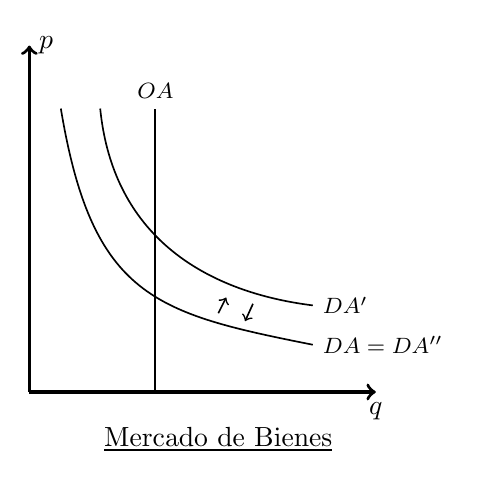
\begin{tikzpicture}[scale=0.4]
\draw[very thick,<-] (0,11)--(0,0);
\draw[very thick,->] (0,0)--(11,0) node[below]{$q$};
\node[right] at (0,11) {$p$};

\node[] at(6,-1.5) {\underline{Mercado de Bienes}};
\draw[semithick] (1,9).. controls (2,3) and (4, 2.5) .. (9, 1.5) node [right]{\footnotesize $DA=DA''$};
\draw[semithick] (2.25,9).. controls (2.75,4) and (7, 3) .. (9, 2.75) node [right]{\footnotesize $DA'$};
\draw[semithick](4, 0)--(4, 9) node [above]{\footnotesize $OA$};
\draw[semithick, ->] (6,2.5)--(6.25,3);
\draw[semithick, <-] (6.85,2.25)--(7.1,2.8);
%\draw[thick, gray, dashed] (4,3)--(0,3);
\end{tikzpicture}
\end{center}
     \end{minipage}
  %  \hfill
    \begin{minipage}[b]{0.45\textwidth}
    \begin{center}
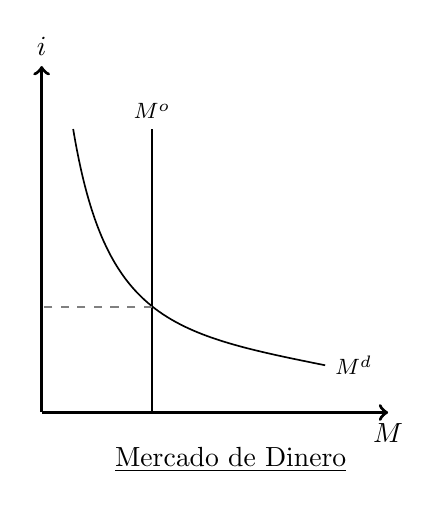
\begin{tikzpicture}[scale=0.4]
\draw[very thick,<-] (0,11) node[above]{$i$}--(0,0);
\draw[very thick,->] (0,0)--(11,0) node[below]{$M$};
\node[right] at (0,11) {};

\node[] at(6,-1.5) {\underline{Mercado de Dinero}};
\draw[semithick] (1,9).. controls (2,3) and (4, 2.5) .. (9, 1.5) node [right]{\footnotesize $M^{d}$};
\draw[semithick](3.5, 0)--(3.5, 9) node [above]{\footnotesize $M^{o}$};

 \draw[thick, gray, dashed] (3.5,3.35)--(0,3.35);

\end{tikzpicture}
\end{center}
    \end{minipage}
\end{center}
\vspace{0.7cm}
\label{fig:C36.2}
\end{figure}
\end{center}   
   
\end{frame}

\begin{frame}{Primer caso. Expansión fiscal con impuestos permanentes}
   Conclusiones:
   \begin{itemize}
       \item No hay efectos: lo que el gobierno gasta, la gente lo deja de gastar.
       \item La demanda agregada no se modifica
       \item No importa como es la curva de oferta
       \item Es decir el resultado es el mismo en el mundo clásico o keynesiano
   \end{itemize}
\end{frame}

\begin{frame}{Expansión fiscal c/ impuestos transitorios/clásico}
   
\begin{center}
\begin{figure}[H]
\renewcommand{\figurename}{Figure}
\begin{center}
    \begin{minipage}[b]{0.45\textwidth}
        \begin{center}
\begin{tikzpicture}[scale=0.4]
\draw[very thick,<-] (0,11)--(0,0)0;
\draw[very thick,->] (0,0)--(11,0) node[below]{$q$};
\node[right] at (0,11) {$p$};
\node[] at(6,-1.5) {\underline{Mercado de Bienes}};
\draw[semithick] (1,9).. controls (2,3) and (4, 2.5) .. (9, 1.5) node [right]{\footnotesize $DA$};
\draw[semithick] (2.25,9).. controls (2.75,4) and (7, 3) .. (9, 2.75) node [right]{\footnotesize $DA'$};
\draw[semithick](4, 0)--(4, 9) node [above]{\footnotesize $OA$};
\draw[thick, gray, dashed] (7.5,3)--(0,3);
\draw[thick, gray, dashed] (4,5)--(0,5);
\draw[fill] (7.5,3) circle [radius =0.11] node[above] {\scriptsize A};
\draw[fill] (4,5) circle [radius =0.11] node[right] {\scriptsize B};
\end{tikzpicture}
\end{center}
     \end{minipage}
  %  \hfill
    \begin{minipage}[b]{0.45\textwidth}
    \begin{center}
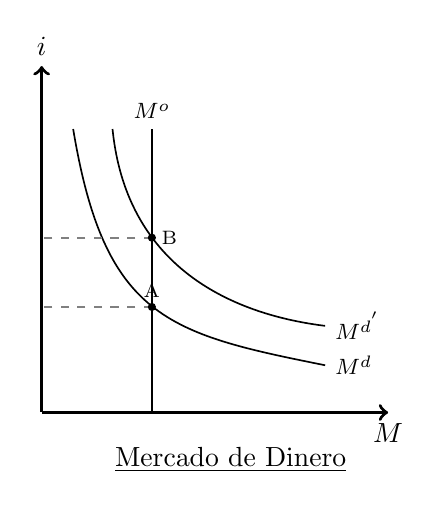
\begin{tikzpicture}[scale=0.4]
\draw[very thick,<-] (0,11) node[above]{$i$}--(0,0);
\draw[very thick,->] (0,0)--(11,0) node[below]{$M$};
\node[right] at (0,11) {};
\node[] at(6,-1.5) {\underline{Mercado de Dinero}};
\draw[semithick] (1,9).. controls (2,3) and (4, 2.5) .. (9, 1.5) node [right]{\footnotesize $M^{d}$};
\draw[semithick] (2.25,9).. controls (2.75,4) and (7, 3) .. (9, 2.75) node [right]{\footnotesize $M^{d^{'}}$};
\draw[semithick](3.5, 0)--(3.5, 9) node [above]{\footnotesize $M^{o}$};
 \draw[thick, gray, dashed] (3.5,3.35)--(0,3.35);
 \draw[thick, gray, dashed] (3.5,5.55)--(0,5.55);
 %\draw[semithick, ->] (6,2.5)--(6.25,3);
%\draw[semithick, <-] (6.85,2.25)--(7.1,2.8);
\draw[fill] (3.5,3.35) circle [radius =0.11] node[above] {\scriptsize A};
\draw[fill] (3.5,5.55) circle [radius =0.11] node[right] {\scriptsize B};

\end{tikzpicture}
\end{center}
    \end{minipage}
\end{center}
\vspace{0.7cm}
\label{fig:C36.2}
\end{figure}
\end{center} 

\end{frame}

%---------------------------------------------------------------------------%
\begin{frame}{Segundo caso. Expansión fiscal c/impuestos transitorios/clásico}
   
\begin{itemize}
    \item La reversión de la demanda agregada no es plena
    \item El exceso de demanda empuja los precios para arriba
    \item Eso aumenta la demanda de dinero empujando para arriba la tasa de interés 
    \item A la postre el crowding out es pleno
    \end{itemize}
\end{frame}

%---------------------------------------------------------------------------%
\begin{frame}{Expansión fiscal c/impuestos transitorios/keynesiano}
    
\begin{center}
\begin{figure}[H]
\renewcommand{\figurename}{Figure}
\begin{center}
    \begin{minipage}[b]{0.45\textwidth}
        \begin{center}
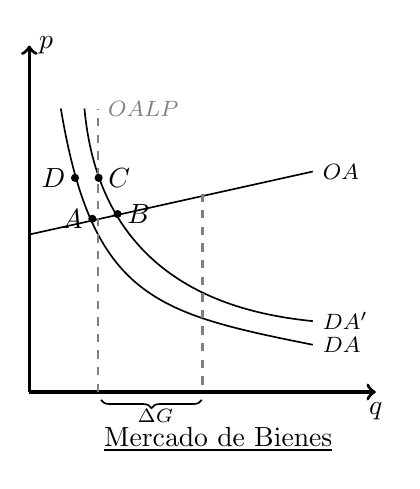
\begin{tikzpicture}[scale=0.4]
\draw[very thick,<-] (0,11)--(0,0);
\draw[very thick,->] (0,0)--(11,0) node[below]{$q$};
\node[right] at (0,11) {$p$};

\node[] at(6,-1.5) {\underline{Mercado de Bienes}};
\draw[semithick] (1,9).. controls (2,3) and (4, 2.5) .. (9, 1.5) node [right]{\footnotesize $DA$};
%\draw[semithick] (2.25,9).. controls (2.75,4) and (7, 3) .. (9, 2.75) node [right]{\footnotesize $DA'$};
\draw[semithick] (1.75,9).. controls (2.25,3.5) and (6.5,2.5) .. (9, 2.25) node [right]{\footnotesize $DA'$};
\draw[semithick](0, 5)--(9, 7) node [right]{\footnotesize $OA$};
\draw [semithick,decorate,decoration={brace,amplitude=3pt, mirror},xshift=5pt,yshift=0pt](2.1,-0.25) -- (5.3,-0.25);
\draw (4,-0.75) node[]{\scriptsize $\Delta G $};
\draw[thick, gray, dashed] (2.175,0)--(2.175,9) node [right]{\footnotesize $OALP$};;
\draw[thick, gray, dashed] (5.5,6.3)--(5.5,0);
\draw[fill] (2,5.5) circle [radius =0.11] node[left] {$A$}; 
\draw[fill] (2.8,5.65) circle [radius =0.11] node[right] {$B$}; 
\draw[fill] (2.2,6.8) circle [radius =0.11] node[right] {$C$}; 
\draw[fill] (1.45,6.8) circle [radius =0.11] node[left] {$D$}; 
\end{tikzpicture}
\end{center}
     \end{minipage}
  %  \hfill
    \begin{minipage}[b]{0.45\textwidth}
    \begin{center}
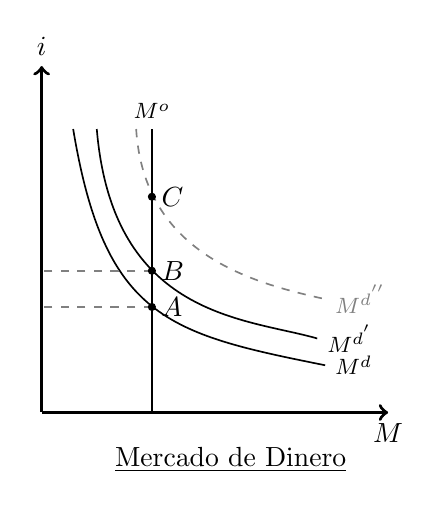
\begin{tikzpicture}[scale=0.4]
\draw[very thick,<-] (0,11) node[above]{$i$}--(0,0);
\draw[very thick,->] (0,0)--(11,0) node[below]{$M$};
\node[right] at (0,11) {};
\node[] at(6,-1.5) {\underline{Mercado de Dinero}};
\draw[semithick] (1,9).. controls (2,3) and (4, 2.5) .. (9, 1.5) node [right]{\footnotesize $M^{d}$};
\draw[semithick] (1.75,9).. controls (2.25,3) and (6.5, 3) .. (8.75, 2.35) node [right]{\footnotesize $M^{d^{'}}$};
\draw[semithick, gray, dashed] (3,9).. controls (3.25,5) and (6.75,4.1) .. (9,3.6) node [right]{\footnotesize $M^{d^{''}}$};
\draw[semithick](3.5, 0)--(3.5, 9) node [above]{\footnotesize $M^{o}$};
\draw[thick, gray, dashed] (3.5,3.35)--(0,3.35);
\draw[thick, gray, dashed] (3.5,4.5)--(0,4.5);
\draw[fill] (3.5,3.35) circle [radius =0.11] node[right] {$A$}; 
\draw[fill] (3.5,4.5) circle [radius =0.11] node[right] {$B$}; 
\draw[fill] (3.5,6.85) circle [radius =0.11] node[right] {$C$};
\end{tikzpicture}
\end{center}
    \end{minipage}
\end{center}
\vspace{0.7cm}
\label{fig:C36.4}
\end{figure}
\end{center} 

\end{frame}

\begin{frame}{Tercer caso. Expansión fiscal c/impuestos transitorios/keynesiano}
   
\begin{itemize}
    \item La reversión de la demanda agregada no es plena
    \item El exceso de demanda hace subir el producto 
    \item Eso aumenta la demanda de dinero empujando para arriba la tasa de interés 
    \item La tasa de interés sube menos (que en el caso clásico) y el producto se expande 
    \item Los precios empiezan  a subir, cuando la politica se revierte, se pasa por una fase recesiva 
\end{itemize}
    
\end{frame}


%---------------------------------------------------------------------------%


\begin{frame}{¿Cómo funciona la política fiscal financiada con deuda doméstica?}

    \begin{itemize}
    \item Acá el punto clave es si los agentes anticipan la carga impositiva que implica la mayor deuda
    \item Si se anticipan los impuestos necesarios para pagar esta deuda, es igual que el caso anterior (equivalencia ricardiana)
    \item En la práctica se encuentra que el ahorro responde a la deuda, pero que la compensación no es plena
    \item En tanto el efecto no es de compensación plena, hay un efecto expansivo en la demanda agregada (con efecto sobre el producto en un mundo keynesiano)

    \end{itemize}

\end{frame}



%---------------------------------------------------------------------------%

%\begin{frame}{Expansión fiscal con deuda no ricardianos, clásico}

%\begin{center}
%\begin{figure}[H]
%\renewcommand{\figurename}{Figure}
%\begin{center}
%    \begin{minipage}[b]{0.45\textwidth}
%        \begin{center}
%\begin{tikzpicture}[scale=0.4]
%\draw[very thick,<-] (0,11)--(0,0);
%\draw[very thick,->] (0,0)--(11,0) node[below]{$q$};
%\node[right] at (0,11) {$p$};

%\node[] at(6,-1.5) {\underline{Mercado de Bienes}};
%\draw[semithick] (1,9).. controls (2,3) and (4, 2.5) .. (9, 1.5) node [right]{\footnotesize $DA$};
%\draw[semithick] (2.25,9).. controls (2.75,4) and (7, 3) .. (9, 2.75) node [right]{\footnotesize $DA'$};
%\draw[semithick] (3.25,9).. controls (3.25,5) and (8.5, 3.75) .. (9, 3.75) node [right]{\footnotesize $DA'''$};
%\draw[semithick](4, 0)--(4, 9) node [above]{\footnotesize $OA$};
%\draw[thick, gray, dashed] (7.5,3)--(0,3);
%\draw[thick, gray, dashed] (4,5)--(0,5);
%\draw[fill] (7.5,3) circle [radius =0.11] node[above] {\scriptsize A};
%\draw[fill] (4,5) circle [radius =0.11] node[right] {\scriptsize B};
%\draw[fill] (4,6.5) circle [radius =0.11] node[left] {\scriptsize C}; 
%\end{tikzpicture}
%\end{center}
 %    \end{minipage}
  %  \hfill
 %   \begin{minipage}[b]{0.45\textwidth}
 %   \begin{center}
%\begin{tikzpicture}[scale=0.4]
%\draw[very thick,<-] (0,11) node[above]{$i$}--(0,0);
%\draw[very thick,->] (0,0)--(11,0) node[below]{$M$};
%\node[right] at (0,11) {};
%\node[] at(6,-1.5) {\underline{Mercado de Dinero}};
%\draw[semithick] (1,9).. controls (2,3) and (4, 2.5) .. (9, 1.5) node [right]{\footnotesize $M^{d}$};
% \draw[semithick] (2.25,9).. controls (2.75,4) and (7, 3) .. (9, 2.75) node [right]{\footnotesize $M^{d^{'}}$};
%\draw[semithick] (1.75,9).. controls (2.25,2.75) and (6.25, 2.75) .. (9, 2.25) node [right]{\footnotesize $M^{d^{'}}$};
%\draw[semithick] (2.25,9).. controls (2.75,4) and (7, 3) .. (9, 2.75) node [right]{\footnotesize $M^{d^{'}}$};
%\draw[semithick](3.5, 0)--(3.5, 9) node [above]{\footnotesize $M^{o}$};
% \draw[semithick](6.5, 0)--(6.5, 9) node [above]{\footnotesize $M^{s}'$};
%  \draw[thick, gray, dashed] (3.5,3.35)--(-3.5,3.35);
%  \draw[thick, gray, dashed] (3.5,5.55)--(-3.5,5.55);
%\draw[thick, gray, dashed] (3.5,3.35)--(0,3.35);
% \draw[thick, gray, dashed] (3.5,5.55)--(0,5.55);
% \draw[thick, gray, dashed] (3.5,4.25)--(0,4.25);
%\draw[fill] (3.5,3.4) circle [radius =0.11] node[right] {\scriptsize A};  
%\draw[fill] (3.5,5.55) circle [radius =0.11] node[left] {\scriptsize B};  
%\draw[fill] (3.5,5.55) circle [radius =0.11] node[right] {\scriptsize B};  
%\end{tikzpicture}
%\end{center}
%    \end{minipage}
%\end{center}
%\vspace{0.7cm}
%\caption{\textbf{Política fiscal financiada con deuda en el mundo clásico}}
%\label{fig:C36.7}
%\end{figure}
%\end{center} 

%\end{frame}




%---------------------------------------------------------------------------%
%\begin{frame}{Expansión fiscal/deuda/ricardianos/clásico}
   
 %  \begin{itemize}
 %      \item La reversión de la demanda agregada es plena y no se modifica
  %     \item Por consiguiente no tenemos efectos en el mercado monetario y de trabajo
   %    \item En el mercado de credito aparece la demanda del gobierno
    %    \item Pero como la gente (ricardiana) anticipa los mayores impuestos aumenta su ahorro en la misma magnitud! 
     %    \item Con lo cual no se modifican las tasas de interés 
     %     \item De hecho una de las pruebas de si hay equivalencia ricardiana es ver si las tasas de interés cambian con el déficit fiscal
   %\end{itemize}
    
%\end{frame}

%\begin{frame}{Expansión fiscal/deuda/no ricardianos/clásico}
   
 
 %  \begin{itemize}
 %      \item La reversión de la demanda agregada no es plena con lo que aumenta 
  
  %     \item Los precios aumentan eliminando el exceso de demanda
   
   
   
   %    \item Esto empuja para arriba la demanda de dinero-
    
%    \item En el mercado de crédito el gobierno aumenta la demanda incrementando la tasa de interés. 
  %       \item Como a la tasa de interés del mercado de crédito hay un exceso de oferta de dinero la tasa de interés se ubica en un valor algo menor. 
   %     \item Pero el crowding out es total
%        \item Porque lo que toma el gobierno es exacto lo que tiene que caer el consumo y la inversión. 
 %        \item En el mercado de trabajo los salarios acompañan a los precios sin efecto en el empleo 
 %  \end{itemize}
    
%\end{frame}

%---------------------------------------------------------------------------%

\begin{frame}{27. Cuarto caso. Expansión fiscal con deuda no ricardianos, keynesiano}


\begin{center}
\begin{figure}[H]
\renewcommand{\figurename}{Figure}
\begin{center}
    \begin{minipage}[b]{0.45\textwidth}
        \begin{center}
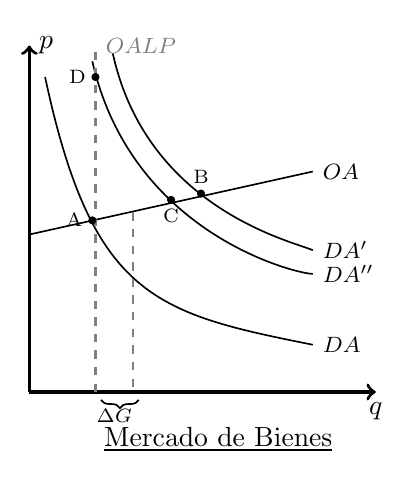
\begin{tikzpicture}[scale=0.4]
\draw[very thick,<-] (0,11)--(0,0);
\draw[very thick,->] (0,0)--(11,0) node[below]{$q$};
\node[right] at (0,11) {$p$};

\node[] at(6,-1.5) {\underline{Mercado de Bienes}};
\draw[semithick] (0.5,10).. controls (2,3) and (4, 2.5) .. (9, 1.5) node [right]{\footnotesize $DA$};

\draw[semithick] (2.65,10.75).. controls (3.75,5.75) and (8.5, 4.75) .. (9, 4.5) node [right]{\footnotesize $DA'$};
\draw[semithick] (2,10.5).. controls (3.25,5) and (8.5, 3.75) .. (9, 3.75) node [right]{\footnotesize $DA''$};
\draw[semithick](0, 5)--(9, 7) node [right]{\footnotesize $OA$};
  \draw [semithick,decorate,decoration={brace,amplitude=3pt, mirror},xshift=5pt,yshift=0pt](2.1,-0.25) -- (3.3,-0.25);
\draw (2.7,-0.75) node[]{\scriptsize $\Delta G $};

 \draw[thick, gray, dashed] (2.1,0)--(2.1,11) node [right]{\footnotesize $OALP$};
\draw[thick, gray, dashed] (3.3,5.7)--(3.3,0); 
\draw[fill] (2,5.45) circle [radius =0.11] node[left] {\scriptsize A};  
\draw[fill] (5.45,6.3) circle [radius =0.11] node[above] {\scriptsize B}; 
\draw[fill] (4.5,6.1) circle [radius =0.11] node[below] {\scriptsize C};  
\draw[fill] (2.1,10) circle [radius =0.11] node[left] {\scriptsize D};  
\end{tikzpicture}
\end{center}
     \end{minipage}
  %  \hfill
    \begin{minipage}[b]{0.45\textwidth}
    \begin{center}
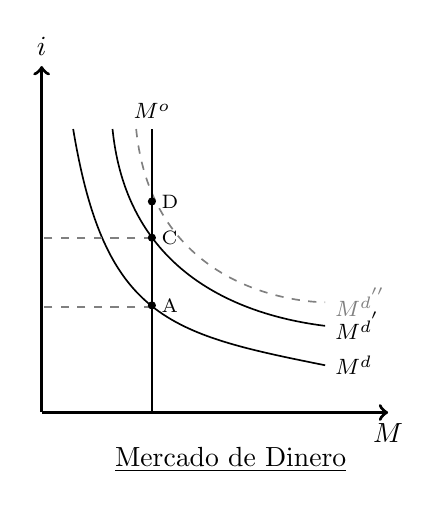
\begin{tikzpicture}[scale=0.4]
\draw[very thick,<-] (0,11) node[above]{$i$}--(0,0);
\draw[very thick,->] (0,0)--(11,0) node[below]{$M$};
\node[right] at (0,11) {};
\node[] at(6,-1.5) {\underline{Mercado de Dinero}};
\draw[semithick] (1,9).. controls (2,3) and (4, 2.5) .. (9, 1.5) node [right]{\footnotesize $M^{d}$};
\draw[semithick] (2.25,9).. controls (2.75,4) and (7, 3) .. (9, 2.75) node [right]{\footnotesize $M^{d^{'}}$};
\draw[semithick, gray, dashed] (3,9).. controls (3.5,4) and (8, 3.5) .. (9,3.5) node [right]{\footnotesize $M^{d^{''}}$};
\draw[semithick](3.5, 0)--(3.5, 9) node [above]{\footnotesize $M^{o}$};
% \draw[thick](6.5, 0)--(6.5, 9) node [above]{\footnotesize $M^{s}'$};

 \draw[thick, gray, dashed] (3.5,3.35)--(0,3.35);
 \draw[thick, gray, dashed] (3.5,5.55)--(0,5.55);
\draw[fill] (3.5,3.4) circle [radius =0.11] node[right] {\scriptsize A};  
\draw[fill] (3.5,5.55) circle [radius =0.11] node[right] {\scriptsize C};  
 \draw[fill] (3.5,6.7) circle [radius =0.11] node[right] {\scriptsize D};  
\end{tikzpicture}
\end{center}
    \end{minipage}
\end{center}
\vspace{0.7cm}
\label{fig:C36.8}
\end{figure}
\end{center} 

\end{frame}



%---------------------------------------------------------------------------%
%\begin{frame}{Expansión fiscal/deuda/no ricardianos/keynesiano}
   
%   \begin{itemize}
 %      \item La reversión de la demanda agregada no es plena con lo que aumenta 
  %     \item Pero los precios no aumentan con lo que sube el producto
   %    \item Esto empuja para arriba la demanda de dinero y la tasa de interés nominal
    %    \item En el mercado de crédito el gobierno aumenta la demanda, el aumento en la demanda de dinero reduce algo la oferta (compensado parcialmente por el aumento del producto) 
     %   \item Acá el equilibrio es con un mayor nivel de crédito, no hay crowding out total porque el producto aumentó! 
      %   \item En el mercado de trabajo los salarios no se mueven y aumenta el empleo  
   %\end{itemize}
    
%\end{frame}


%---------------------------------------------------------------------------%

%---------------------------------------------------------------------------%
%\begin{frame}{Expansión fiscal/deuda externa/no ricardianos/keynesiano}
%    \begin{center}
%\begin{figure}[H]
%\renewcommand{\figurename}{Figure}
%\begin{center}
%\begin{tikzpicture}[scale=0.29]
%\draw[very thick,<->] (0,11) node[left]{$w$}--(0,0)--(-11,0) node[below]{$T$};
%\draw[very thick,->] (0,0)--(11,0) node[below]{$q$};
%\node[right] at (0,11) {$p$};

%\node[] at(-5,11.5) {\underline{Mercado de Trabajo}};
%\draw[semithick] (-1,9).. controls (-2,3) and (-4, 2.5) .. (-9, 1.5) node [left]{\footnotesize $DT$};
%\draw[semithick] (-2.25,9).. controls (-2.75,4) and (-7, 3) .. (-9, 2.75) node [left]{\footnotesize $DT'$};
%\draw[semithick](0,5)--(-7, 5)--(-7, 9) node [above]{\footnotesize $OT$};

%\node[] at(6,11.5) {\underline{Mercado de Bienes}};
%\draw[semithick] (1,9).. controls (2,3) and (4, 2.5) .. (9, 1.5) node [right]{\footnotesize $DA$};
%\draw[semithick] (2.25,9).. controls (2.75,4) and (7, 3) .. (9, 2.75) node [right]{\footnotesize $DA'$};
%\draw[semithick](0, 5)--(9, 5) node [right]{\footnotesize $OA$};
%   \draw [semithick,decorate,decoration={brace,amplitude=3pt, mirror},xshift=5pt,yshift=0pt](2.1,-0.25) -- (5.3,-0.25);
% \draw (4,-0.75) node[]{\scriptsize $\Delta G $};

% \draw[thick, gray, dashed] (2.175,5)--(2.175,0);
% \draw[thick, gray, dashed] (5.5,5)--(5.5,0);
%\end{tikzpicture}



%\begin{tikzpicture}[scale=0.29]
%\draw[very thick,<->] (0,11) node[above]{$i$}--(0,0)--(-11,0) node[below]{$FP$};
%\draw[very thick,->] (0,0)--(11,0) node[below]{$M$};
%\node[right] at (0,11) {};

%\node[] at(-5,-1.5) {\underline{Mercado de Crédito}};
%\draw[semithick] (-1,9).. controls (-2,3) and (-4, 2.5) .. (-9, 1.5) node [left]{\footnotesize $D_{FP}$};
%\draw[semithick] (-2.25,9).. controls (-2.75,4) and (-7, 3) .. (-9, 2.75) node [left]{\footnotesize $D_{FP}'$};
%\draw[thick,dashed] (-3.5,9)--(-3.5,0) node [below]{\footnotesize 0};

%\node[] at(6,-1.5) {\underline{Mercado de Dinero}};
%\draw[semithick] (1,9).. controls (2,3) and (4, 2.5) .. (9, 1.5) node [right]{\footnotesize $M^{d}$};
%\draw[semithick] (2.25,9).. controls (2.75,4) and (7, 3) .. (9, 2.75) node [right]{\footnotesize $M^{d^{'}}$};
%\draw[semithick](3.5, 0)--(3.5, 9) node [above]{\footnotesize $M^{o}$};
%\draw[semithick](6.5, 0)--(6.5, 9) node [above]{\footnotesize $M^{s^{'}}$};
% \draw[thick](6.5, 0)--(6.5, 9) node [above]{\footnotesize $M^{s}'$};

% \draw[thick, gray, dashed] (6.5,3.35)--(-3.5,3.35);
% \draw[thick, gray, dashed] (3.5,5.55)--(-3.5,5.55);

%\end{tikzpicture}
%\end{center}
%\vspace{0.7cm}
%\caption{\textbf{La política fiscal financiada con deuda externa y agentes no ricardianos en el mundo keynesiano}}
%\label{fig:C36.8}
%\end{figure}
%\end{center}


%\end{frame}

%---------------------------------------------------------------------------%

%\begin{frame}{Expansión fiscal/deuda externa/no ricardianos/keynesiano}
   
 %  \begin{itemize}
%       \item La reversión de la demanda agregada no es plena con lo que aumenta 
%       \item Los precios no aumentan empujando hacia arriba el producto
%       
%        \item En el mercado de crédito el gobierno aumenta la demanda, pero ojo: ahora ese aumento viene con su oferta (la deuda externa). No hay un aumento en la demanda neta.
%        \item El credito actua como aumentando los medios de pagos.
 
% \item En el mercado de trabajo los salarios no se mueven y el aumento en la demanda agregada aumenta el empleo 
% \item Es el más expansivo de los casos que vimos.
%   \end{itemize}
    
%\end{frame}

%---------------------------------------------------------------------------%

\begin{frame}{Discusión}

    \begin{itemize}
    \item Para un clásico hay poco por hacer: más vale concentrarte en lo estructural: competencia, apertura, instituciones
    \item En el mundo keynesiano, al menos hay margen, pero…
    \item A) La mayor parte de los cambios en el producto son generados por cambios en C e I, causados por los agentes individuales, inducidos por el ambiente político y las expectativas
    \item B) ¿Estamos seguros el gobierno será efectivo o incluso si actuará cuando debe actuar? 
    \end{itemize}

\end{frame}

%---------------------------------------------------------------------------%

\begin{frame}{Caveats a la política macroeconómica}

    \begin{itemize}
    \item Puede existir un problema de rezagos: las políticas pueden hacerse en un momento inadecuado
    \item Podes pensar que podes cuando no podes (si el mundo es clásico, las políticas sólo van a resultar en inflación o deflación)
    \item Si el marco político genera gobiernos débiles, puede existir prociclicalidad fiscal o exceso de gasto
    \item Las políticas pueden incrementar la incertidumbre
    \item La gente puede anticipar estas políticas haciéndolas menos efectivas (inconsistencia temporal y expectativas racionales), por ejemplo si vos aumentas el dinero y la gente se da cuenta al toque, los precios suben y no lográs nada
    \end{itemize}

\end{frame}


%\begin{frame}{Sustentabilidad Fiscal}

 %   \begin{itemize}
 %   \item Decimos que una deuda es no-sustentable si vemos que el ratio deuda PBI sube
  %   \item La deuda crece a la tasa r
  %    \item El PBI crece a la tasa g
  %     \item Decimos que la deuda esta en una trayectoria no sustentable si  
   %     \item Superávit primario (ingresos menos gastos excluyendo intereses) es menor que (r-g) Deuda/PBI. 
%     \item En Argentina por ejemplo la deuda externa era 40\% del PBI. r=5.5\% y g= 4\%. Esto implica que el déficit primario requerido era 0.6\% del PBI. 
 %   \item Pero el déficit primario recibido era 0.4\% así que no había un gran tema.
 %   \item Ahorro? 40\% sobre 100. 000 millones. 40.000 millones. En realidad 20.000 porque la mitad la tenían argentinos
 %    \item Efecto sobre el valor del capital privado: 150.000 millones
  %  \end{itemize}

%\end{frame}


\begin{frame}{Las tipologías de la macro}
\begin{table}[]
\resizebox{\textwidth}{!}{%
\begin{tabular}{|c|c|c|}
\hline
           & Shock a la oferta                                                                      & Shock a la demanda           \\ \hline
Clasico    & Teoria del ciclo real                                                                  & Inefectividad de la politica \\ \hline
Keynesiano & \begin{tabular}[c]{@{}c@{}}Conflicto entre estabilidad\\ y estabilización\end{tabular} & Divina coincidencia          \\ \hline
\end{tabular}%
}
\end{table}

\end{frame}



\begin{frame}{¿Cómo funciona la política fiscal?}
    \begin{itemize}
        \item El análisis de la política fiscal es mucho más complejo por una serie de motivos:
        \begin{itemize}
            \item La política fiscal expansiva genera aumentos de la demanda agregada 
            \item Pero la política fiscal requiere financiamiento
            \begin{itemize}
                \item Necesitamos entender cómo puede financiar el Gobierno para hacer uso de este instrumento
            \end{itemize}
            \item Hay efectos expulsión (“crowding out”) vía la tasa de interés (que no aparecían con la política monetaria)
        \end{itemize}
        \vspace{2mm}
        \item La combinación de estos tres factores nos dará el efecto neto de la política fiscal sobre la demanda agregada
    \end{itemize}
\end{frame}

\begin{frame}{¿Cómo puede financiar el gasto un gobierno?}
    \begin{itemize}
        \item Existen cuatro mecanismos básicos para financiar la política fiscal:
        \begin{itemize}
            \item Hacer emisión monetaria 
            \item Aumentar los impuestos
            \item Pedir deuda interna
            \item Pedir deuda externa 
        \end{itemize}
        \vspace{2mm}
        \item Cada uno de estos implicará distintos mecanismos sobre la demanda agregada
    \end{itemize}
\end{frame}

\begin{frame}{El efecto “financiamiento” sobre el consumo}
    \begin{itemize}
        \item Supongamos primero que aumenta el gasto público financiado enteramente con impuestos: ¿cuánto cae el consumo privado?
        \begin{itemize}
            \item Depende de si los impuestos son permanentes o transitorios
            \item Si los impuestos son permanentes la caída del consumo debiera ser igual al aumento de los impuestos
            \item La caída del consumo es menor si se piensa que el aumento de impuestos es transitorio
            \item Lo cierto es que el efecto de la política fiscal se modera sustancialmente cuando se tiene en cuenta el financiamiento
        \end{itemize}
    \end{itemize}
\end{frame}

\begin{frame}{Primer caso: Expansión fiscal con impuestos permanentes (caso clásico)}
 
\begin{figure}[H]
\renewcommand{\figurename}{Figure}
\begin{center}
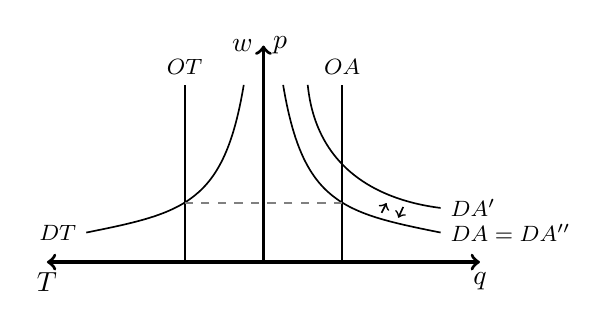
\begin{tikzpicture}[scale=0.25]
\draw[very thick,<->] (0,11) node[left]{$w$}--(0,0)--(-11,0) node[below]{$T$};
\draw[very thick,->] (0,0)--(11,0) node[below]{$q$};
\node[right] at (0,11) {$p$};

%\node[] at(-5,11.5) {\underline{Mercado de Trabajo}};
\draw[semithick] (-1,9).. controls (-2,3) and (-4, 2.5) .. (-9, 1.5) node [left]{\footnotesize $DT$};
%\draw[semithick] (-2.25,9).. controls (-2.75,4) and (-7, 3) .. (-9, 2.75) node [left]{\footnotesize $DT'$};
\draw[semithick](-4, 0)--(-4, 9) node [above]{\footnotesize $OT$};

%\node[] at(6,11.5) {\underline{Mercado de Bienes}};
\draw[semithick] (1,9).. controls (2,3) and (4, 2.5) .. (9, 1.5) node [right]{\footnotesize $DA=DA''$};
\draw[semithick] (2.25,9).. controls (2.75,4) and (7, 3) .. (9, 2.75) node [right]{\footnotesize $DA'$};
\draw[semithick](4, 0)--(4, 9) node [above]{\footnotesize $OA$};

\draw[semithick, ->] (6,2.5)--(6.25,3);
\draw[semithick, <-] (6.85,2.25)--(7.1,2.8);


\draw[thick, gray, dashed] (4,3)--(-4,3);
%\draw[thick, gray, dashed] (4,5)--(-4,5);

\end{tikzpicture}



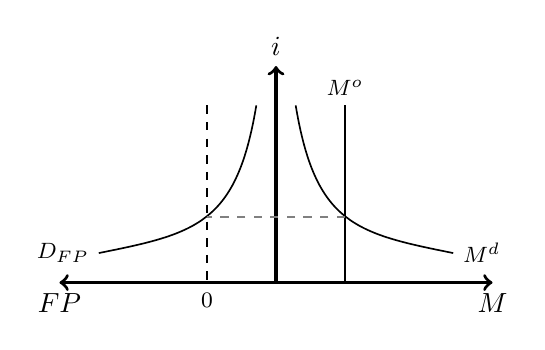
\begin{tikzpicture}[scale=0.25]
\draw[very thick,<->] (0,11) node[above]{$i$}--(0,0)--(-11,0) node[below]{$FP$};
\draw[very thick,->] (0,0)--(11,0) node[below]{$M$};
\node[right] at (0,11) {};

%\node[] at(-5,-1.5) {\underline{Mercado de Crédito}};
\draw[semithick] (-1,9).. controls (-2,3) and (-4, 2.5) .. (-9, 1.5) node [left]{\footnotesize $D_{FP}$};
%\draw[semithick] (-2.25,9).. controls (-2.75,4) and (-7, 3) .. (-9, 2.75) node [left]{\footnotesize $D_{FP}'$};
\draw[thick,dashed] (-3.5,9)--(-3.5,0) node [below]{\footnotesize 0};


%\node[] at(6,-1.5) {\underline{Mercado de Dinero}};
\draw[semithick] (1,9).. controls (2,3) and (4, 2.5) .. (9, 1.5) node [right]{\footnotesize $M^{d}$};
%\draw[semithick] (2.25,9).. controls (2.75,4) and (7, 3) .. (9, 2.75) node [right]{\footnotesize $M^{d^{'}}$};
\draw[semithick](3.5, 0)--(3.5, 9) node [above]{\footnotesize $M^{o}$};
% \draw[thick](6.5, 0)--(6.5, 9) node [above]{\footnotesize $M^{s}'$};

 \draw[thick, gray, dashed] (3.5,3.35)--(-3.5,3.35);
% \draw[thick, gray, dashed] (4,5)--(-4,5);

\end{tikzpicture}
\end{center}
\vspace{0.7cm}
\caption{\textbf{Política fiscal financiada con un aumento permanente de los impuestos}}
\label{fig:C36.2}
\end{figure}
\end{frame}

\begin{frame}{Primer caso: Expansión fiscal con impuestos permanentes (caso clásico)}
   Conclusiones:
   \begin{itemize}
       \item No hay efectos: lo que el gobierno gasta, la gente lo deja de gastar.
       \item La demanda agregada no se modifica
       \item No importa como es la curva de oferta
       \item Es decir el resultado es el mismo en el mundo clásico o keynesiano
   \end{itemize}
\end{frame}

\begin{frame}{Segundo caso: Expansión fiscal con impuestos transitorios (caso clásico)}
   
\begin{center}
\begin{figure}[H]
\renewcommand{\figurename}{Figure}
\begin{center}
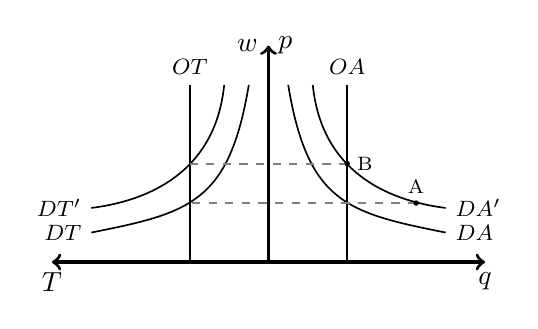
\begin{tikzpicture}[scale=0.25]
\draw[very thick,<->] (0,11) node[left]{$w$}--(0,0)--(-11,0) node[below]{$T$};
\draw[very thick,->] (0,0)--(11,0) node[below]{$q$};
\node[right] at (0,11) {$p$};

%\node[] at(-5,11.5) {\underline{Mercado de Trabajo}};
\draw[semithick] (-1,9).. controls (-2,3) and (-4, 2.5) .. (-9, 1.5) node [left]{\footnotesize $DT$};
\draw[semithick] (-2.25,9).. controls (-2.75,4) and (-7, 3) .. (-9, 2.75) node [left]{\footnotesize $DT'$};
\draw[semithick](-4, 0)--(-4, 9) node [above]{\footnotesize $OT$};

%\node[] at(6,11.5) {\underline{Mercado de Bienes}};
\draw[semithick] (1,9).. controls (2,3) and (4, 2.5) .. (9, 1.5) node [right]{\footnotesize $DA$};
\draw[semithick] (2.25,9).. controls (2.75,4) and (7, 3) .. (9, 2.75) node [right]{\footnotesize $DA'$};
\draw[semithick](4, 0)--(4, 9) node [above]{\footnotesize $OA$};

\draw[thick, gray, dashed] (7.5,3)--(-4,3);
\draw[thick, gray, dashed] (4,5)--(-4,5);
\draw[fill] (7.5,3) circle [radius =0.11] node[above] {\scriptsize A};
\draw[fill] (4,5) circle [radius =0.11] node[right] {\scriptsize B};
\end{tikzpicture}



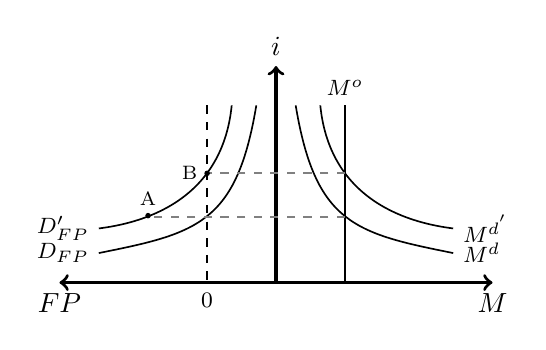
\begin{tikzpicture}[scale=0.25]
\draw[very thick,<->] (0,11) node[above]{$i$}--(0,0)--(-11,0) node[below]{$FP$};
\draw[very thick,->] (0,0)--(11,0) node[below]{$M$};
\node[right] at (0,11) {};

%\node[] at(-5,-1.5) {\underline{Mercado de Crédito}};
\draw[semithick] (-1,9).. controls (-2,3) and (-4, 2.5) .. (-9, 1.5) node [left]{\footnotesize $D_{FP}$};
\draw[semithick] (-2.25,9).. controls (-2.75,4) and (-7, 3) .. (-9, 2.75) node [left]{\footnotesize $D_{FP}'$};
\draw[thick,dashed] (-3.5,9)--(-3.5,0) node [below]{\footnotesize 0};


%\node[] at(6,-1.5) {\underline{Mercado de Dinero}};
\draw[semithick] (1,9).. controls (2,3) and (4, 2.5) .. (9, 1.5) node [right]{\footnotesize $M^{d}$};
\draw[semithick] (2.25,9).. controls (2.75,4) and (7, 3) .. (9, 2.75) node [right]{\footnotesize $M^{d^{'}}$};
\draw[semithick](3.5, 0)--(3.5, 9) node [above]{\footnotesize $M^{o}$};
% \draw[semithick](6.5, 0)--(6.5, 9) node [above]{\footnotesize $M^{s}'$};

 \draw[thick, gray, dashed] (3.5,3.35)--(-6.5,3.35);
 \draw[thick, gray, dashed] (3.5,5.55)--(-3.5,5.55);
\draw[fill] (-6.5,3.4) circle [radius =0.11] node[above] {\scriptsize A};  
\draw[fill] (-3.5,5.55) circle [radius =0.11] node[left] {\scriptsize B};  

\end{tikzpicture}
\end{center}
\vspace{0.7cm}
\caption{\textbf{Política fiscal financiada con un aumento transitorio de los impuestos - Clásico}}
\label{fig:C36.3}
\end{figure}
\end{center}
\end{frame}

\begin{frame}{Segundo caso: Expansión fiscal con impuestos transitorios (caso clásico)}
    Conclusiones:
   \begin{itemize}
       \item La reversión de la demanda agregada no es plena
       \item El exceso de demanda empuja los precios para arriba
       \item Eso aumenta la demanda de dinero empujando para arriba la tasa de interés
       \item En el mercado de crédito aumenta la demanda (la gente quiere suavizar el consumo) y cae la oferta (los bancos tiene menos M para prestar)
       \item El salario nominal sube acompañando los precios 
    \item En definitiva: el crowding out es pleno
    \end{itemize}
\end{frame}

\begin{frame}{Segundo caso: Expansión fiscal con impuestos transitorios (caso keynesiano)}
\begin{figure}[H]
\renewcommand{\figurename}{Figure}
\begin{center}
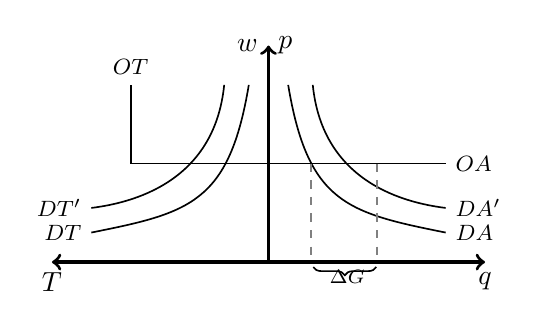
\begin{tikzpicture}[scale=0.25]
\draw[very thick,<->] (0,11) node[left]{$w$}--(0,0)--(-11,0) node[below]{$T$};
\draw[very thick,->] (0,0)--(11,0) node[below]{$q$};
\node[right] at (0,11) {$p$};

%\node[] at(-5,11.5) {\underline{Mercado de Trabajo}};
\draw[semithick] (-1,9).. controls (-2,3) and (-4, 2.5) .. (-9, 1.5) node [left]{\footnotesize $DT$};
\draw[semithick] (-2.25,9).. controls (-2.75,4) and (-7, 3) .. (-9, 2.75) node [left]{\footnotesize $DT'$};
\draw[semithick](0,5)--(-7, 5)--(-7, 9) node [above]{\footnotesize $OT$};

%\node[] at(6,11.5) {\underline{Mercado de Bienes}};
\draw[semithick] (1,9).. controls (2,3) and (4, 2.5) .. (9, 1.5) node [right]{\footnotesize $DA$};
\draw[semithick] (2.25,9).. controls (2.75,4) and (7, 3) .. (9, 2.75) node [right]{\footnotesize $DA'$};
\draw[semithick](0, 5)--(9, 5) node [right]{\footnotesize $OA$};

  \draw [semithick,decorate,decoration={brace,amplitude=3pt, mirror},xshift=5pt,yshift=0pt](2.1,-0.25) -- (5.3,-0.25);
\draw (4,-0.75) node[]{\scriptsize $\Delta G $};

\draw[thick, gray, dashed] (2.175,5)--(2.175,0);
\draw[thick, gray, dashed] (5.5,5)--(5.5,0);
\end{tikzpicture}

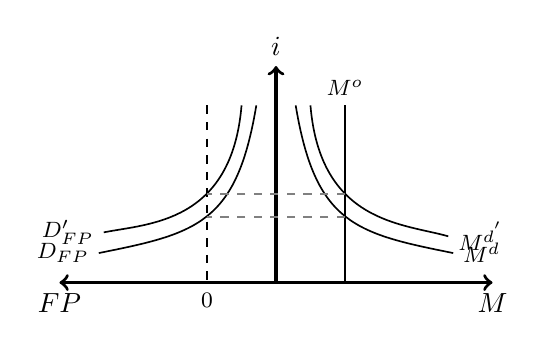
\begin{tikzpicture}[scale=0.25]
\draw[very thick,<->] (0,11) node[above]{$i$}--(0,0)--(-11,0) node[below]{$FP$};
\draw[very thick,->] (0,0)--(11,0) node[below]{$M$};
\node[right] at (0,11) {};

%\node[] at(-5,-1.5) {\underline{Mercado de Crédito}};
\draw[semithick] (-1,9).. controls (-2,3) and (-4, 2.5) .. (-9, 1.5) node [left]{\footnotesize $D_{FP}$};
\draw[semithick] (-1.75,9).. controls (-2.25,3) and (-6.5, 3) .. (-8.75, 2.55) node [left]{\footnotesize $D_{FP}'$};
\draw[thick,dashed] (-3.5,9)--(-3.5,0) node [below]{\footnotesize 0};

%\node[] at(6,-1.5) {\underline{Mercado de Dinero}};
\draw[semithick] (1,9).. controls (2,3) and (4, 2.5) .. (9, 1.5) node [right]{\footnotesize $M^{d}$};
%\draw[semithick] (2.25,9).. controls (2.75,4) and (7, 3) .. (9, 2.75) node [right]{\footnotesize $M^{d^{'}}$};
\draw[semithick] (1.75,9).. controls (2.25,3) and (6.5, 3) .. (8.75, 2.35) node [right]{\footnotesize $M^{d^{'}}$};
\draw[semithick](3.5, 0)--(3.5, 9) node [above]{\footnotesize $M^{o}$};
% \draw[thick](6.5, 0)--(6.5, 9) node [above]{\footnotesize $M^{s}'$};

 \draw[thick, gray, dashed] (3.5,3.35)--(-3.5,3.35);
 \draw[thick, gray, dashed] (3.5,4.5)--(-3.5,4.5);

\end{tikzpicture}
\end{center}
\vspace{0.7cm}
\caption{\textbf{Política fiscal financiada con un aumento transitorio de los impuestos - Keynesiano}}
\label{fig:C36.4}
\end{figure}

\end{frame}

\begin{frame}{Segundo caso: Expansión fiscal con impuestos transitorios (caso keynesiano)}
   Conclusiones:
   \begin{itemize}
       \item La reversión de la demanda agregada no es plena
       \item El exceso de demanda hace subir el producto 
       \item Eso aumenta la demanda de dinero empujando para arriba la tasa de interés 
       \item En el mercado de crédito aumenta la demanda (la gente quiere suavizar el consumo) y cae la oferta (los bancos tiene menos M para prestar)
       \item La caída de la oferta es menor que en el mundo clásico (porque aumenta el producto)
       \item El salario nominal no se mueve y sube el empleo
        \item La tasa de interés sube menos (que en el caso clásico) y el producto se expande 
   \end{itemize}
    
\end{frame}

\begin{frame}{El efecto “financiamiento” sobre el consumo}
    \begin{itemize}
        \item Supongamos ahora que aumenta el gasto público financiado con deuda: ¿cuánto cae el consumo privado?
        \begin{itemize}
            \item En principio podríamos pensar que nada (agentes no ricardianos)
            \item Pero en realidad, si existe “equivalencia ricardiana” es igual que si financia con impuestos
            \item Y hay crowding out también si hay un aumento en la tasa de interés
        \end{itemize}
    \end{itemize}
\end{frame}

\begin{frame}{¿Qué es la equivalencia ricardiana?}
    \begin{itemize}
        \item Supongamos dos periodos y un consumidor que tiene ingresos de 1000 y 1000
        \item El gobierno va a gastar 100 y 100 
        \begin{itemize}
            \item Lo financia con deuda en el primer periodo y la tasa de interés es 10\% y con impuestos en el segundo periodo
            \item El agente enfrenta impuestos de 0 en el primer periodo y 210 en el segundo periodo (100 de impuestos y 110 de lo que se endeudo el gobierno)
            \item Si consume su ingreso, consumiría 1000 en el primer periodo y 790 en el segundo periodo 
        \end{itemize}
        \item ¿Qué pasa si ahorra 100 en el primero período?
        \begin{itemize}
        \item Ahora puede consumir 900 y 900 (porque en le segundo periodo tiene 110 que proviene de lo que ahorró)
        \item Eso es mejor que 1000 y 790 porque quiere suavizar consumo
        \end{itemize}
        \item Pero 900 y 900 es lo mismo que si el gobierno hubiera financiado los 100 con impuestos!!! 
\end{itemize}
\end{frame}

\begin{frame}{¿Pero existe ese fenómeno Ricardiano? I}
     \begin{center}
         Correlación entre deuda pública y activos financieros netos acumulados por los hogares
     \end{center}
     \centering\includegraphics[width=11cm]{P91b.png}\  
     \begin{center}
         Grennes y Strazds (2013) en base a datos de Eurostat
     \end{center}
\end{frame}

\begin{frame}{¿Pero existe ese fenómeno Ricardiano? II}
     \centering\includegraphics[width=11cm]{Figures/C36.11.png}\  
\begin{itemize}
    \item El caso sudafricano reciente
    \end{itemize}
\end{frame}

\begin{frame}{¿Qué es el efecto expulsión o “crowding out”?}
    \begin{itemize}
    \footnotesize\item El efecto expulsión tiene dos componentes:
        \begin{itemize}
        \scriptsize\item El menor ingreso neto del consumidor (porque aumentan los impuestos) implica menor ahorro lo cual reduce la oferta de fondos prestables
        \scriptsize\item La mayor demanda de fondos públicos del consumidor (si pide deuda) aumenta la demanda de fondos prestables sube la tasa de interés y por ende debilita la inversión
        \scriptsize\end{itemize}
    \end{itemize}
    \vspace{0.2cm}
    \centering\includegraphics[width=7cm]{P87.png}\
\end{frame}

\begin{frame}{El efecto expulsión en un mundo ricardiano}
    \begin{itemize}
    \scriptsize\item A menos que el financiamiento genere un aumento del ahorro privado
    \scriptsize\item Por ejemplo, un aumento del gasto publico financiado con deuda en un contexto Ricardiano no afecta la inversión porque la tasa no cambia
    \scriptsize\item Pero la caída del consumo diluye el efecto sobre la demanda agregada
    \end{itemize}
    
    \vspace{0.2cm}
    
    \centering\includegraphics[width=7cm]{P88.png}\

\end{frame}

\begin{frame}{Tercer caso: Expansión fiscal financiada con deuda doméstica}
    \begin{itemize}
    \item Acá el punto clave es si los agentes anticipan la carga impositiva que implica la mayor deuda
    \item Si se anticipan los impuestos necesarios para pagar esta deuda, es igual que el caso anterior (equivalencia ricardiana)
    \item En la práctica se encuentra que el ahorro responde a la deuda, pero que la compensación no es plena
    \item En tanto el efecto no es de compensación plena, hay un efecto expansivo en la demanda agregada (con efecto sobre el producto en un mundo keynesiano)

    \end{itemize}

\end{frame}

\begin{frame}{Cuarto caso: Expansión fiscal financiado con deuda e individuos no ricardianos (caso clásico)}
    \begin{figure}
\begin{center}
\begin{figure}[H]
\renewcommand{\figurename}{Figure}
\begin{center}
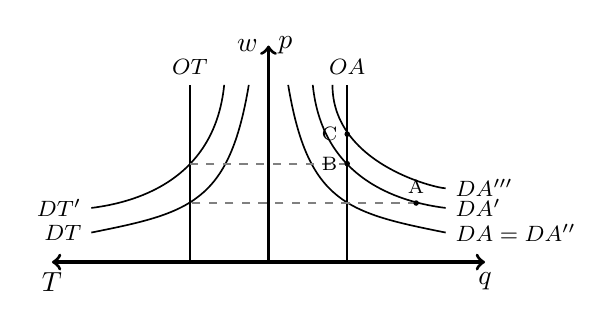
\begin{tikzpicture}[scale=0.25]
\draw[very thick,<->] (0,11) node[left]{$w$}--(0,0)--(-11,0) node[below]{$T$};
\draw[very thick,->] (0,0)--(11,0) node[below]{$q$};
\node[right] at (0,11) {$p$};

%\node[] at(-5,11.5) {\underline{Mercado de Trabajo}};
\draw[semithick] (-1,9).. controls (-2,3) and (-4, 2.5) .. (-9, 1.5) node [left]{\footnotesize $DT$};
\draw[semithick] (-2.25,9).. controls (-2.75,4) and (-7, 3) .. (-9, 2.75) node [left]{\footnotesize $DT'$};
\draw[semithick](-4, 0)--(-4, 9) node [above]{\footnotesize $OT$};

%\node[] at(6,11.5) {\underline{Mercado de Bienes}};
\draw[semithick] (1,9).. controls (2,3) and (4, 2.5) .. (9, 1.5) node [right]{\footnotesize $DA=DA''$};
\draw[semithick] (2.25,9).. controls (2.75,4) and (7, 3) .. (9, 2.75) node [right]{\footnotesize $DA'$};
\draw[semithick] (3.25,9).. controls (3.25,5) and (8.5, 3.75) .. (9, 3.75) node [right]{\footnotesize $DA'''$};
%\draw[semithick] (1.5,9).. controls (2.5,3) and (6, 2.75) .. (9, 2.1) node [right]{\footnotesize $DA'''$};
\draw[semithick](4, 0)--(4, 9) node [above]{\footnotesize $OA$};

% \draw[thick, gray, dashed] (4,3)--(-4,3);
% \draw[thick, gray, dashed] (4,5)--(-4,5);


\draw[thick, gray, dashed] (7.5,3)--(-4,3);
\draw[thick, gray, dashed] (4,5)--(-4,5);
\draw[fill] (7.5,3) circle [radius =0.11] node[above] {\scriptsize A};
\draw[fill] (4,5) circle [radius =0.11] node[left] {\scriptsize B};
\draw[fill] (4,6.5) circle [radius =0.11] node[left] {\scriptsize C};

\end{tikzpicture}



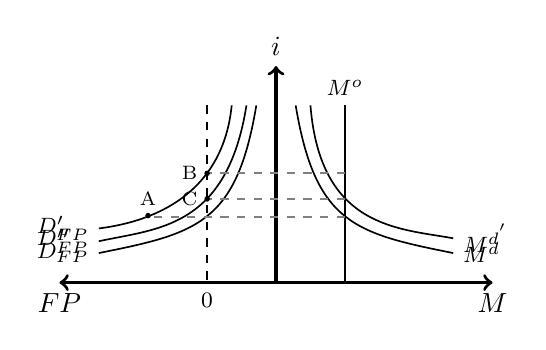
\begin{tikzpicture}[scale=0.25]
\draw[very thick,<->] (0,11) node[above]{$i$}--(0,0)--(-11,0) node[below]{$FP$};
\draw[very thick,->] (0,0)--(11,0) node[below]{$M$};
\node[right] at (0,11) {};

%\node[] at(-5,-1.5) {\underline{Mercado de Crédito}};
\draw[semithick] (-1,9).. controls (-2,3) and (-4, 2.5) .. (-9, 1.5) node [left]{\footnotesize $D_{FP}$};
\draw[semithick] (-2.25,9).. controls (-2.75,4) and (-7, 3) .. (-9, 2.75) node [left]{\footnotesize $D_{FP}'$};
\draw[semithick] (-1.5,9).. controls (-2.5,2.75) and (-6, 2.75) .. (-9, 2.1) node [left]{\footnotesize $D_{FP}''$};
\draw[thick,dashed] (-3.5,9)--(-3.5,0) node [below]{\footnotesize 0};

%\node[] at(6,-1.5) {\underline{Mercado de Dinero}};
\draw[semithick] (1,9).. controls (2,3) and (4, 2.5) .. (9, 1.5) node [right]{\footnotesize $M^{d}$};
% \draw[semithick] (2.25,9).. controls (2.75,4) and (7, 3) .. (9, 2.75) node [right]{\footnotesize $M^{d^{'}}$};
\draw[semithick] (1.75,9).. controls (2.25,2.75) and (6.25, 2.75) .. (9, 2.25) node [right]{\footnotesize $M^{d^{'}}$};
\draw[semithick](3.5, 0)--(3.5, 9) node [above]{\footnotesize $M^{o}$};
% \draw[semithick](6.5, 0)--(6.5, 9) node [above]{\footnotesize $M^{s}'$};

%  \draw[thick, gray, dashed] (3.5,3.35)--(-3.5,3.35);
%  \draw[thick, gray, dashed] (3.5,5.55)--(-3.5,5.55);

 \draw[thick, gray, dashed] (3.5,3.35)--(-6.5,3.35);
 \draw[thick, gray, dashed] (3.5,5.55)--(-3.5,5.55);
 \draw[thick, gray, dashed] (3.5,4.25)--(-3.5,4.25);
\draw[fill] (-6.5,3.4) circle [radius =0.11] node[above] {\scriptsize A};  
\draw[fill] (-3.5,5.55) circle [radius =0.11] node[left] {\scriptsize B};  
\draw[fill] (-3.5,4.25) circle [radius =0.11] node[left] {\scriptsize C};  

\end{tikzpicture}
\end{center}
\vspace{0.7cm}
\caption{\textbf{Política fiscal financiada con deuda en el mundo clásico}}
\label{fig:C36.5}
\end{figure}
\end{center}

  \begin{center}  

  \begin{tikzpicture}[trim axis left,
    scale=1.4,
    axis/.style={ultra thick, ->, >=stealth'},
    important line/.style={ultra thick},
    dashed line/.style={dashed, thin},
    pile/.style={thick, ->, >=stealth', shorten <=2pt, shorten
    >=2pt},
    every node/.style={color=black}
    ]
    
     % Axis
     \draw[axis] (0,0)  -- (2,0) node(xline)[below, text width=2em]
        {\textbf{$Q$}};
    \draw[axis] (0,0) -- (0,2) node(yline)[above] {$P$};
    % Lines
    \draw[important line] (1,0)  -- (1,2) ;
    \draw[important line] (0.2,1.6)-- (1.6,0.2);
    \draw[important line,red] (0.2,2.2)-- (2.2,0.2);
\end{tikzpicture}
\qquad
\begin{tikzpicture}[trim axis left,
    scale=1.4,
    axis/.style={ultra thick, ->, >=stealth'},
    important line/.style={ultra thick},
    dashed line/.style={dashed, thin},
    pile/.style={thick, ->, >=stealth', shorten <=2pt, shorten
    >=2pt},
    every node/.style={color=black}
    ]
    
     % Axis
     \draw[axis] (0,0)  -- (2,0) node(xline)[below, text width=2em]
        {\textbf{$M$}};
    \draw[axis] (0,0) -- (0,2) node(yline)[above] {$i$};
    % Lines
    \draw[important line] (1,0)  -- (1,2) ;
    \draw[important line] (0.2,1.6)-- (1.6,0.2);
\end{tikzpicture}
\\
\begin{tikzpicture}[trim axis left,
    scale=1.4,
    axis/.style={ultra thick, ->, >=stealth'},
    important line/.style={ultra thick},
    dashed line/.style={dashed, thin},
    pile/.style={thick, ->, >=stealth', shorten <=2pt, shorten
    >=2pt},
    every node/.style={color=black}
    ]
    
     % Axis
     \draw[axis] (0,0)  -- (2,0) node(xline)[below,text width=2em]
        {\textbf{$C$}};
    \draw[axis] (0,0) -- (0,2) node(yline)[above] {$r$};
    % Lines
    \draw[important line] (0.4,0.2)  -- (1.8,1.6) ;
    \draw[important line] (0.2,1.6)-- (1.6,0.2);
        \draw[important line, blue] (1,0.2)  -- (2.4,1.6) ;
    \draw[important line, blue] (0.2,2.2)-- (2.2,0.2);
    \draw[dashed] (0,0.8)--(2,.8);
\end{tikzpicture}
\qquad
\begin{tikzpicture}[trim axis left,
    scale=1.4,
    axis/.style={ultra thick, ->, >=stealth'},
    important line/.style={ultra thick},
    dashed line/.style={dashed, thin},
    pile/.style={thick, ->, >=stealth', shorten <=2pt, shorten
    >=2pt},
    every node/.style={color=black}
    ]
    
     % Axis
     \draw[axis] (0,0)  -- (2,0) node(xline)[below,text width=2em]{\textbf{$L$}};
    \draw[axis] (0,0) -- (0,2) node(yline)[above] {$w$};
    % Lines
    \draw[important line] (1,0)  -- (1,2) ;
    \draw[important line] (0.2,1.6)-- (1.6,0.2);
\end{tikzpicture}
\end{center}
\end{figure}
\end{frame}

\begin{frame}{Cuarto caso: Expansión fiscal financiado con deuda e individuos no ricardianos (caso clásico)}
   
   \begin{itemize}
       \item La reversión de la demanda agregada no es plena con lo que aumenta 
       \item Los precios aumentan eliminando el exceso de demanda
       \item Esto empuja para arriba la demanda de dinero-
        \item En el mercado de crédito el gobierno aumenta la demanda incrementando la tasa de interés. 
         \item Como a la tasa de interés del mercado de crédito hay un exceso de oferta de dinero la tasa de interés se ubica en un valor algo menor. 
        \item Pero el crowding out es total
        \item Porque lo que toma el gobierno es exacto lo que tiene que caer el consumo y la inversión. 
         \item En el mercado de trabajo los salarios acompañan a los precios sin efecto en el empleo 
   \end{itemize}
    
\end{frame}

\begin{frame}{Cuarto caso: Expansión fiscal financiado con deuda e individuos no ricardianos (caso keynesiano)}
    \begin{center}
\begin{figure}[H]
\renewcommand{\figurename}{Figure}
\begin{center}
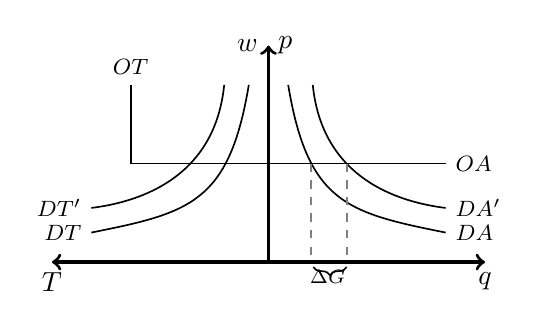
\begin{tikzpicture}[scale=0.25]
\draw[very thick,<->] (0,11) node[left]{$w$}--(0,0)--(-11,0) node[below]{$T$};
\draw[very thick,->] (0,0)--(11,0) node[below]{$q$};
\node[right] at (0,11) {$p$};

%\node[] at(-5,11.5) {\underline{Mercado de Trabajo}};
\draw[semithick] (-1,9).. controls (-2,3) and (-4, 2.5) .. (-9, 1.5) node [left]{\footnotesize $DT$};
\draw[semithick] (-2.25,9).. controls (-2.75,4) and (-7, 3) .. (-9, 2.75) node [left]{\footnotesize $DT'$};
\draw[semithick](0,5)--(-7, 5)--(-7, 9) node [above]{\footnotesize $OT$};

%\node[] at(6,11.5) {\underline{Mercado de Bienes}};
\draw[semithick] (1,9).. controls (2,3) and (4, 2.5) .. (9, 1.5) node [right]{\footnotesize $DA$};
\draw[semithick] (2.25,9).. controls (2.75,4) and (7, 3) .. (9, 2.75) node [right]{\footnotesize $DA'$};
\draw[semithick](0, 5)--(9, 5) node [right]{\footnotesize $OA$};
  \draw [semithick,decorate,decoration={brace,amplitude=3pt, mirror},xshift=5pt,yshift=0pt](2.1,-0.25) -- (3.8,-0.25);
\draw (3,-0.75) node[]{\scriptsize $\Delta G $};

\draw[thick, gray, dashed] (2.175,5)--(2.175,0);
\draw[thick, gray, dashed] (4,5)--(4,0);
\end{tikzpicture}



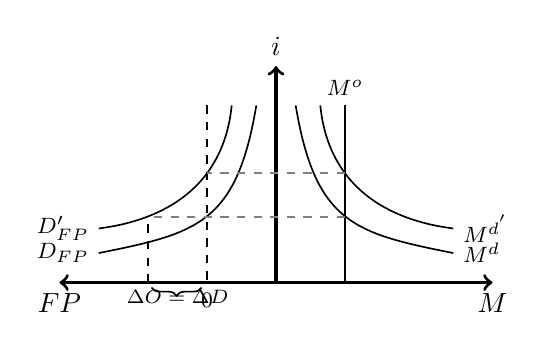
\begin{tikzpicture}[scale=0.25]
\draw[very thick,<->] (0,11) node[above]{$i$}--(0,0)--(-11,0) node[below]{$FP$};
\draw[very thick,->] (0,0)--(11,0) node[below]{$M$};
\node[right] at (0,11) {};

%\node[] at(-5,-1.5) {\underline{Mercado de Crédito}};
\draw[semithick] (-1,9).. controls (-2,3) and (-4, 2.5) .. (-9, 1.5) node [left]{\footnotesize $D_{FP}$};
\draw[semithick] (-2.25,9).. controls (-2.75,4) and (-7, 3) .. (-9, 2.75) node [left]{\footnotesize $D_{FP}'$};
\draw[thick,dashed] (-3.5,9)--(-3.5,0) node [below]{\footnotesize 0};
\draw[thick, dashed] (-6.5,0)--(-6.5,3.35);
  \draw [semithick,decorate,decoration={brace,amplitude=3pt, mirror},xshift=5pt,yshift=0pt](-6.5,-0.25) -- (-3.95,-0.25);
\draw (-5,-0.75) node[]{\scriptsize $\Delta O = \Delta D $};

%\node[] at(6,-1.5) {\underline{Mercado de Dinero}};
\draw[semithick] (1,9).. controls (2,3) and (4, 2.5) .. (9, 1.5) node [right]{\footnotesize $M^{d}$};
\draw[semithick] (2.25,9).. controls (2.75,4) and (7, 3) .. (9, 2.75) node [right]{\footnotesize $M^{d^{'}}$};
\draw[semithick](3.5, 0)--(3.5, 9) node [above]{\footnotesize $M^{o}$};
% \draw[thick](6.5, 0)--(6.5, 9) node [above]{\footnotesize $M^{s}'$};

 \draw[thick, gray, dashed] (3.5,3.35)--(-6.5,3.35);
 \draw[thick, gray, dashed] (3.5,5.55)--(-3.5,5.55);

\end{tikzpicture}
\end{center}
\vspace{0.7cm}
\caption{\textbf{Política fiscal financiada con deuda en el mundo keynesiano}}
\label{fig:C36.7}
\end{figure}
\end{center}
\end{frame}

\begin{frame}{Cuarto caso: Expansión fiscal financiado con deuda e individuos no ricardianos (caso keynesiano)}
   
   \begin{itemize}
       \item La reversión de la demanda agregada no es plena con lo que aumenta 
       \item Pero los precios no aumentan con lo que sube el producto
       \item Esto empuja para arriba la demanda de dinero y la tasa de interés nominal
        \item En el mercado de crédito el gobierno aumenta la demanda, el aumento en la demanda de dinero reduce algo la oferta (compensado parcialmente por el aumento del producto) 
        \item Acá el equilibrio es con un mayor nivel de crédito, no hay crowding out total porque el producto aumentó! 
         \item En el mercado de trabajo los salarios no se mueven y aumenta el empleo  
   \end{itemize}
    
\end{frame}

\begin{frame}{Cuarto caso: Expansión fiscal financiado con deuda e individuos no ricardianos (caso keynesiano)}
    \begin{center}
\begin{figure}[H]
\renewcommand{\figurename}{Figure}
\begin{center}
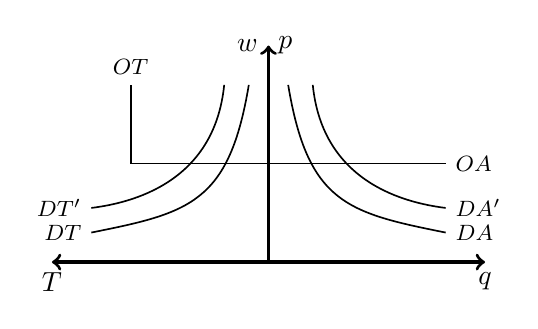
\begin{tikzpicture}[scale=0.25]
\draw[very thick,<->] (0,11) node[left]{$w$}--(0,0)--(-11,0) node[below]{$T$};
\draw[very thick,->] (0,0)--(11,0) node[below]{$q$};
\node[right] at (0,11) {$p$};

%\node[] at(-5,11.5) {\underline{Mercado de Trabajo}};
\draw[semithick] (-1,9).. controls (-2,3) and (-4, 2.5) .. (-9, 1.5) node [left]{\footnotesize $DT$};
\draw[semithick] (-2.25,9).. controls (-2.75,4) and (-7, 3) .. (-9, 2.75) node [left]{\footnotesize $DT'$};
\draw[semithick](0,5)--(-7, 5)--(-7, 9) node [above]{\footnotesize $OT$};

%\node[] at(6,11.5) {\underline{Mercado de Bienes}};
\draw[semithick] (1,9).. controls (2,3) and (4, 2.5) .. (9, 1.5) node [right]{\footnotesize $DA$};
\draw[semithick] (2.25,9).. controls (2.75,4) and (7, 3) .. (9, 2.75) node [right]{\footnotesize $DA'$};
\draw[semithick](0, 5)--(9, 5) node [right]{\footnotesize $OA$};
%   \draw [semithick,decorate,decoration={brace,amplitude=3pt, mirror},xshift=5pt,yshift=0pt](2.1,-0.25) -- (5.3,-0.25);
% \draw (4,-0.75) node[]{\scriptsize $\Delta G $};

% \draw[thick, gray, dashed] (2.175,5)--(2.175,0);
% \draw[thick, gray, dashed] (5.5,5)--(5.5,0);
\end{tikzpicture}



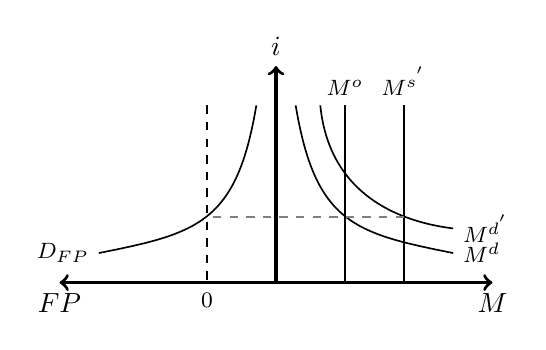
\begin{tikzpicture}[scale=0.25]
\draw[very thick,<->] (0,11) node[above]{$i$}--(0,0)--(-11,0) node[below]{$FP$};
\draw[very thick,->] (0,0)--(11,0) node[below]{$M$};
\node[right] at (0,11) {};

%\node[] at(-5,-1.5) {\underline{Mercado de Crédito}};
\draw[semithick] (-1,9).. controls (-2,3) and (-4, 2.5) .. (-9, 1.5) node [left]{\footnotesize $D_{FP}$};
%\draw[semithick] (-2.25,9).. controls (-2.75,4) and (-7, 3) .. (-9, 2.75) node [left]{\footnotesize $D_{FP}'$};
\draw[thick,dashed] (-3.5,9)--(-3.5,0) node [below]{\footnotesize 0};

%\node[] at(6,-1.5) {\underline{Mercado de Dinero}};
\draw[semithick] (1,9).. controls (2,3) and (4, 2.5) .. (9, 1.5) node [right]{\footnotesize $M^{d}$};
\draw[semithick] (2.25,9).. controls (2.75,4) and (7, 3) .. (9, 2.75) node [right]{\footnotesize $M^{d^{'}}$};
\draw[semithick](3.5, 0)--(3.5, 9) node [above]{\footnotesize $M^{o}$};
\draw[semithick](6.5, 0)--(6.5, 9) node [above]{\footnotesize $M^{s^{'}}$};
% \draw[thick](6.5, 0)--(6.5, 9) node [above]{\footnotesize $M^{s}'$};

 \draw[thick, gray, dashed] (6.5,3.35)--(-3.5,3.35);
% \draw[thick, gray, dashed] (3.5,5.55)--(-3.5,5.55);

\end{tikzpicture}
\end{center}
\vspace{0.7cm}
\caption{\textbf{La política fiscal financiada con deuda externa y agentes no ricardianos en el mundo keynesiano}}
\label{fig:C36.8}
\end{figure}
\end{center}


\end{frame}

\begin{frame}{Cuarto caso: Expansión fiscal financiado con deuda e individuos no ricardianos (caso keynesiano)}
   
   \begin{itemize}
       \item La reversión de la demanda agregada no es plena con lo que aumenta 
       \item Los precios no aumentan empujando hacia arriba el producto
       
        \item En el mercado de crédito el gobierno aumenta la demanda, pero ojo: ahora ese aumento viene con su oferta (la deuda externa). No hay un aumento en la demanda neta.
        \item El credito actua como aumentando los medios de pagos.
 
 \item En el mercado de trabajo los salarios no se mueven y el aumento en la demanda agregada aumenta el empleo 
 \item Es el más expansivo de los casos que vimos.
   \end{itemize}
    
\end{frame}

\begin{frame}{¿Cuándo tiene, entonces, la política fiscal un efecto sobre la demanda agregada?}

    \begin{itemize}
    \item Cuando no hay una reducción equivalente del consumo privado.
    \end{itemize}
     \vspace{3mm}
    
    \centering\includegraphics[width=6cm]{P95b.png}\

\end{frame}

\begin{frame}{Discusión}

    \begin{itemize}
    \item Para un clásico hay poco por hacer: más vale concentrarte en lo estructural: competencia, apertura, instituciones
    \item En el mundo keynesiano, al menos hay margen, pero…
    \item A) La mayor parte de los cambios en el producto son generados por cambios en C e I, causados por los agentes individuales, inducidos por el ambiente político y las expectativas
    \item B) ¿Estamos seguros que el gobierno será efectivo o incluso si actuará cuando debe actuar? 
    \end{itemize}

\end{frame}

\begin{frame}{Caveats a la política macroeconómica}

    \begin{itemize}
    \item Puede existir un problema de rezagos: las políticas pueden hacerse en un momento inadecuado
    \item Podes pensar que podes cuando no podes (si el mundo es clásico, las políticas sólo van a resultar en inflación o deflación)
    \item Si el marco político genera gobiernos débiles, puede existir prociclicalidad fiscal o exceso de gasto
    \item Las políticas pueden incrementar la incertidumbre
    \item La gente puede anticipar estas políticas haciéndolas menos efectivas (inconsistencia temporal y expectativas racionales), por ejemplo si vos aumentas el dinero y la gente se da cuenta al toque, los precios suben y no lográs nada
    \end{itemize}

\end{frame}




\begin{frame}{Sustentabilidad Fiscal}

    \begin{itemize}
    \item Decimos que una deuda es no-sustentable si vemos que el ratio deuda PBI sube
     \item La deuda crece a la tasa r
      \item El PBI crece a la tasa g
       \item Decimos que la deuda esta en una trayectoria no sustentable si  
        \item Superávit primario (ingresos menos gastos excluyendo intereses) es menor que (r-g) Deuda/PBI. 
     \item En Argentina por ejemplo la deuda externa era 40\% del PBI. r=5.5\% y g= 4\%. Esto implica que el déficit primario requerido era 0.6\% del PBI. 
    \item Pero el déficit primario recibido era 0.4\% así que no había un gran tema.
    \item Ahorro? 40\% sobre 100. 000 millones. 40.000 millones. En realidad 20.000 porque la mitad la tenían argentinos
     \item Efecto sobre el valor del capital privado: 150.000 millones
    \end{itemize}

\end{frame}

\begin{frame}{Las tipologías de la macro}
\begin{table}[]
\resizebox{\textwidth}{!}{%
\begin{tabular}{|c|c|c|}
\hline
           & Shock a la oferta                                                                      & Shock a la demanda           \\ \hline
Clasico    & Teoria del ciclo real                                                                  & Inefectividad de la politica \\ \hline
Keynesiano & \begin{tabular}[c]{@{}c@{}}Conflicto entre estabilidad\\ y estabilización\end{tabular} & Divina coincidencia          \\ \hline
\end{tabular}%
}
\end{table}

\end{frame}


\end{document}